%---------change this every homework
\def\yourid{mst3k}
\def\collabs{list your collaborators here}
\def\sources{list your sources here}
% -----------------------------------------------------
\def\duedate{October 2, 2024 at 11:59p}
\def\pnumber{4}
%-------------------------------------

\documentclass[10pt]{article}
\usepackage{dsa2}
\usepackage{tikz-cd}
\usepackage{wrapfig}


\begin{document}
\thispagestyle{empty}
\handout
%%%%%%%%%%%%%%%%%%%%%%%%%%%%%%%%%%%%%%%%%%%%%%%%%%%%%%%%

\begin{problem} Halloween Candy Redux \end{problem}

Professor Bloomfield's kids are trying a new strategy to maximize their Halloween candy haul.  They are still restricted to a fixed number of blocks, $n$, that they can travel in any direction from their house.  However, now they are going to recruit other kids in the neighborhood in a pyramid scheme.  The other kids they recruit will "share" half of their candy, and keep half.

We will assume that Professor Bloomfield, with kids in tow, has moved to a city whose streets are a grid.  The city is big enough that we can assume that the grid extends forever in any direction.  We'll assume each streets gives out the same amount of candy: 1 piece per street.  Our running time is how many streets we cover, so it's the same as the amount of candy collected.

\begin{wrapfigure}{r}{0.5\textwidth}
\begin{center}
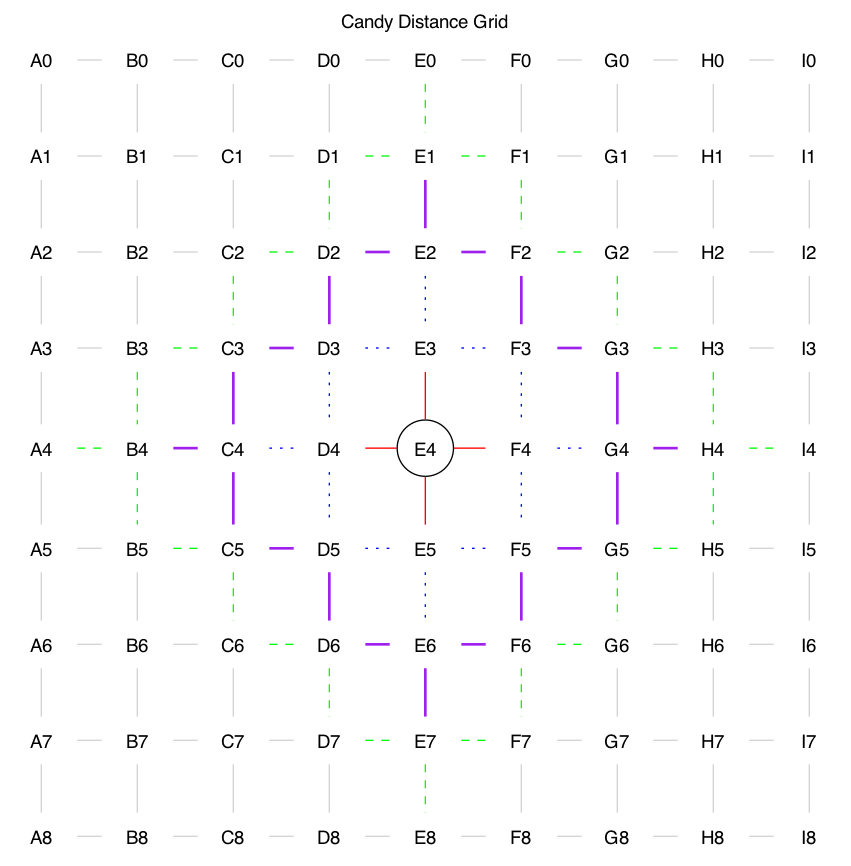
\includegraphics[width=3in]{ps4-graph.png}
\end{center}
\end{wrapfigure}

Consider the graph to the right -- the house (starting location) is at node E4.  If $n=1$, meaning the kids could only go one block, then they would be able to cover the streets indicated by the solid red edges (the ones connecting to node E4).  For $n=2$, it's the solid red and dotted blue edges.  For $n=3$ it also includes the bold purple edges, and for $n=4$ it's also the dashed green edges.  The total number of streets covered, for $n=1,2,3,4$ is $4,16,36,64$.

For this problem you {\bf MUST} use the Master Theorem.  State which case each one is, and show that it fulfills the requirements for that case.

\vspace{0.25in}

\noindent a) Given a value for $n$, which is how many blocks a kid can travel in any direction, how many streets can s/he cover?  This is your $f(n)$ in the $T(n)=a \ast T(n/b) + f(n)$ function.

\solution{

}


\vspace{0.25in}

\noindent Check that $f(n)$ function! If you get it wrong, the rest of your answers will be wrong. Make sure that it really produce the correct results?  For $n=1,2,3,4$ it should yield $4,16,36,64$.

\vspace{0.25in}

\noindent b) Assume that each of his kids recruits four other kids, and each of the other kids can only go half as far.  Note that the other kid will pass back half of the candy collected.  Each of the other kids recruits yet more kids in a similar manner.  How much candy is collected? Write the recurrence relation, show which case of the Master Method applies, then solve using the Master Method.

\solution{

}

\vspace{0.25in}

\noindent c) Now assume that Professor Bloomfield's kids get {\em all} the candy collected by the other kids; each of the other kids can go half as far, and still recruits yet other kids.  How much candy is collected? Write the recurrence relation, show which case of the Master Method applies, then solve using the Master Method.

\solution{

}

\vspace{0.25in}

\noindent d) Lastly, to really expand their operation, each of Professor Bloomfield's kids will recruit 8 other kids, each of which can go half as far and recruits yet other kids.  They are still getting {\em all} the candy collected by the other kids.  How much candy is collected? Write the recurrence relation, show which case of the Master Method applies, then solve using the Master Method.

\solution{

}

%%%%%%%%%%%%%%%%%%%%%%%%%%%%%%%%%%%%%%%%%%%%%%%%%%%%%%%%
\begin{problem}Candy From The Lawnies \end{problem}

It has been a UVA tradition to invite children to come and trick-or-treat on the Lawn. Children dress up in costumes and go from one room to the next collecting candy from inhabitants of the historic Lawn rooms. Professor Bloomfield's children have pressured him in to taking them again this year. Last year things got out of hand when his children went to rooms out-of-order, skipping some, while stopping at others. The children said that they were only choosing to go to rooms that had the best candy. However, it did seem rude to Prof. Bloomfield for his children to walk by some rooms and totally ignore the residents. So the family came up with a heavily negotiated plan for this year. The children can choose any room to start at and any room to stop at, but must visit all rooms in between as well. The children do have access to a secret children's only website that has up-to-the-minute data on the quality of candy given out from every location on Halloween night. All Lawn rooms are listed in the normal walking ordering from the main entrance to the exit, and each room has a candy rating, noted as an integer value from -10 (really bad candy, maybe even a toothbrush) to 10 (the best candy). The children need a plan to achieve the highest candy rating sum possible.


\begin{table}[]
\centering
\begin{tabular}{lllll}
\hline
Entrance &  &  &  &  \\ \hline
Room 1   &  7 &  &  &  \\
Room 2   &  -3 &  &  &  \\
Room 3   &  5 &  &  &  \\
Room 4   &  -4 &  &  &  \\
Room 5   &  2 &  &  &  \\ \hline
Exit   &  &  &  &  \\
\hline
\end{tabular}
\caption{A small example is given in this table. There are only 5 rooms, each with a candy rating. The rooms have an ordering 1-5. In this example, the children could choose to start with any room, then visit additional rooms in order until they want to stop. So they have the following legal choices along with the resulting candy value for each possible choice: [1,2,3,4,5]:7, [1,2,3,4]:5, [2,3,4,5]:0, [1,2,3]:9, [2,3,4]:-2, [3,4,5]:3, [1,2]:4, [2,3]:2, [3,4]:1, [4,5]-2, [1]:7, [2]:-3, [3]:5, [4]-4, or [5]:2. So the best choice in this example is to start with Room 1 and stop after Room 3. }
\end{table}

This problem could be solved in many different ways. As Prof. Bloomfield has recently been teaching his children about divide-and-conquer algorithms, they decide to create a D\&C solution.

Your task is to create a divide and conquer algorithm that solves this problem in $\Theta(n \log n)$ time.

The inputs to your algorithm will be $n$, the number of rooms, $c$ the list that stores the value of candy quality for each of the rooms. Each of the $c$ values is in the range (-10,10). Your algorithm will output the largest sum of candy quality that can be collected based on the constraints described above.

\vspace{0.25in}

What is the divide step for your algorithm?

\solution{

}
\vspace{0.25in}

What is the base case(s)?

\solution{

}
\vspace{0.25in}

What work is done in dividing?

\solution{

}
\vspace{0.25in}

What work is done in combining?

\solution{

}
\vspace{0.25in}

What recursive subproblems are solved?

\solution{

}
\vspace{0.25in}

Make a brief but convincing argument that the time complexity is $\Theta(n \log n)$.

\solution{

}


%%%%%%%%%%%%%%%%%%%%%%%%%%%%%%%%%%%%%%%%%%%%%%%%%%%%%%%%
\end{document}
